%\documentclass[12pt]{scrbook}
%
%\usepackage{tikz}
%\usepackage{minted}
%\usetikzlibrary{decorations.pathreplacing,arrows}
%\usetikzlibrary{arrows,decorations.pathmorphing,backgrounds,positioning,fit,petri}
%
%\usepackage{fullpage}
%\usepackage{subfigure}
%\begin{document}
%
%
%Lorem Ipsum is simply dummy text of the printing and typesetting industry. Lorem Ipsum has been the industry's standard dummy text ever since the 1500s, when an unknown printer took a galley of type and scrambled it to make a type specimen book. It has survived not only five centuries, but also the leap into electronic typesetting, remaining essentially unchanged. It was popularised in the 1960s with the release of Letraset sheets containing Lorem Ipsum passages, and more recently with desktop publishing software like Aldus PageMaker including versions of Lorem Ipsum.





\begin{figure}
\centering

\subfigure[First iteration.  In this partitioning, 2 is the pivot element.
The index variable $i$ is not incremented as 4 is larger than the pivot.
The index variable $j$ decrements to 0 and they are swapped.]{

\begin{tikzpicture}[scale=.65,transform shape]

%\tikzset{>=stealth',shorten <=.2cm,>=stealth',shorten >=.2cm}
% size of each node
\def\sz{9mm}
% node style definition
\tikzstyle{block} = [
	draw, fill=black!10, rectangle,
	minimum height=\sz, minimum width=\sz ];
\tikzstyle{plain} = [draw=none,fill=none];

\node[block,fill=green!50] (a0) at (0*\sz,0) { 2 };
\node[block] (a1) at (1*\sz,0) { 4 };
\node[block] (a2) at (2*\sz,0) { 9 };
\node[block] (a3) at (3*\sz,0) { 4 };
\node[block] (a4) at (4*\sz,0) { 0 };
\node[block] (a5) at (5*\sz,0) { 34 };
\node[block] (a6) at (6*\sz,0) { 12 };

\node[below of=a1] (c1) {};
\draw[->] (c1) -- (a1);

\node[below of=a4] (d4) {};
\draw[->] (d4) -- (a4);
\node[below of=a5] (d5) {};
\draw[->] (d5) -- (a5);
\node[below of=a6] (d6) {};
\draw[->] (d6) -- (a6);
\draw[<-,dotted] (d4) -- (d5);
\draw[<-,dotted] (d5) -- (d6);
\node[below of=d4,above] {$j$};
\node[below of=c1,above] {$i$};

%\draw [decorate,decoration={brace,mirror,amplitude=5pt},xshift=-4pt,yshift=0pt] ([xshift=0cm,yshift=0cm]c1.south) -- ([xshift=0cm,yshift=0cm]c4.south) node [black,midway,yshift=-0.75cm] {$i$};

\draw[<->,>=stealth',shorten <=.2cm,>=stealth',shorten >=.2cm] (a1.south) to [bend right] node[pos=.5,below] {swap} (a4.south);

%\draw[<->] (a4.south) to [in=270,out=270,looseness=1] node[pos=.5,below] {swap} (a8.south);

\end{tikzpicture}~~~~~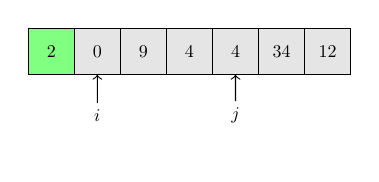
\begin{tikzpicture}[scale=.65,transform shape]

\def\sz{9mm}
\tikzstyle{block} = [
	draw, fill=black!10, rectangle,
	minimum height=\sz, minimum width=\sz ];
\tikzstyle{plain} = [draw=none,fill=none];
\draw[white] (0,0) rectangle (1, -2);

\node[block,fill=green!50] (a0) at (0*\sz,0) { 2 };
\node[block] (a1) at (1*\sz,0) { 0 };
\node[block] (a2) at (2*\sz,0) { 9 };
\node[block] (a3) at (3*\sz,0) { 4 };
\node[block] (a4) at (4*\sz,0) { 4 };
\node[block] (a5) at (5*\sz,0) { 34 };
\node[block] (a6) at (6*\sz,0) { 12 };

\node[below of=a1,node distance=1.25cm] (c4) {$i$};
\draw[->] (c4) -- (a1);
\node[below of=a4,node distance=1.25cm] (d1) {$j$};
\draw[->] (d1) -- (a4);

\end{tikzpicture}

}

\subfigure[Second iteration.  The index variable $i$ is incremented
once, while $j$ is decremented to meet it.  After the while loop the
second case applies as $a_i = 9 > 2 = pivot$, and so we swap 
$a_{i-1} = 2$ with the pivot.]{

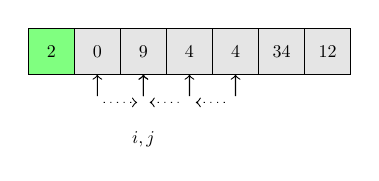
\begin{tikzpicture}[scale=.65,transform shape]

%\tikzset{>=stealth',shorten <=.2cm,>=stealth',shorten >=.2cm}
% size of each node
\def\sz{9mm}
% node style definition
\tikzstyle{block} = [
	draw, fill=black!10, rectangle,
	minimum height=\sz, minimum width=\sz ];
\tikzstyle{plain} = [draw=none,fill=none];

\node[block,fill=green!50] (a0) at (0*\sz,0) { 2 };
\node[block] (a1) at (1*\sz,0) { 0 };
\node[block] (a2) at (2*\sz,0) { 9 };
\node[block] (a3) at (3*\sz,0) { 4 };
\node[block] (a4) at (4*\sz,0) { 4 };
\node[block] (a5) at (5*\sz,0) { 34 };
\node[block] (a6) at (6*\sz,0) { 12 };

\node[below of=a1] (c1) {};
\draw[->] (c1) -- (a1);
\node[below of=a2] (c2) {};
\draw[->] (c2) -- (a2);
\draw[->,dotted] (c1) -- (c2);

\node[below of=a2] (d2) {};
\draw[->] (d2) -- (a2);
\node[below of=a3] (d3) {};
\draw[->] (d3) -- (a3);
\node[below of=a4] (d4) {};
\draw[->] (d4) -- (a4);
\draw[<-,dotted] (d3) -- (d4);
\draw[<-,dotted] (d2) -- (d3);
\node[below of=c2,above] {$i,j$};


%\draw[<->,>=stealth',shorten <=.2cm,>=stealth',shorten >=.2cm] (a1.south) to [bend right] node[pos=.5,below] {swap} (a4.south);

\end{tikzpicture}~~~~~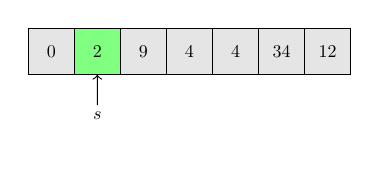
\begin{tikzpicture}[scale=.65,transform shape]

\def\sz{9mm}
\tikzstyle{block} = [
	draw, fill=black!10, rectangle,
	minimum height=\sz, minimum width=\sz ];
\tikzstyle{plain} = [draw=none,fill=none];
\draw[white] (0,0) rectangle (1, -2);

\node[block] (a0) at (0*\sz,0) { 0 };
\node[block,fill=green!50] (a1) at (1*\sz,0) { 2 };
\node[block] (a2) at (2*\sz,0) { 9 };
\node[block] (a3) at (3*\sz,0) { 4 };
\node[block] (a4) at (4*\sz,0) { 4 };
\node[block] (a5) at (5*\sz,0) { 34 };
\node[block] (a6) at (6*\sz,0) { 12 };

\node[below of=a1,node distance=1.25cm] (c4) {$s$};
\draw[->] (c4) -- (a1);

\end{tikzpicture}

}

\caption[Partitioning Example 2]{Example execution of the \textsc{Partition}
subroutine in Quick Sort on the first recursive call on the left partition.  
A total of 6 comparisons are made, 7 if you count the last swap outside the 
while loop.  The partition returns $s$ as the pivot position; in this case
the left-partition is sorted as it only consists of 1 element.}
\label{figure:partitionExample2}

\end{figure}


%\end{document}

